\section{Bezpieczeństwo danych i aplikacji}
\label{sec:bezpieczenstwo}

Tworząc aplikację która będzie używana przez duża grupę obiorców, oprócz osób z pełnymi uprawnieniami do dowolnej akcji również osoby które nie powinny mieć możliwości zmiany danych należy przewidzieć i przygotować odpowiedni zbiór ról i uprawnień. Dostęp do dostarczanych funkcjonalności należy zapewnić poprzez zbiór ról i uprawnień.

Do prawidłowego działania przewidziano kilka ról których obecność ma na celu zabezpieczenie systemu przed nieautoryzowanym dostęp, zmianą jego kodu źródłowego lub edycją danych do których użytkownik nie ma dostępu. Poniżej przedstawiono spis osób, ról które istnieją na końcowym etapie, właściwym działaniu na produkcyjnym środowisku.

\begin{itemize}
\item
Administrator

Osoba która posiada dostęp do serwera na krórym działa aplikacja korzystająca z omawianego frameworku. Ponieważ tworzony program jest jedynie narzędziem służącym do pracy z interaktywnymi mapami, a jednym z założeń jest jak największa adaptabliność i mozliwość działania na różnych środowiskach wymagana jest osoba która doda do działającej strony aplikację.
\item
Moderator

Pzygotowanie i edycja map powinna być wykonana przez uprawnione osoby. Może to być na przykład osoba posiadającą dużą wiedzę na dany temat, posiada ona możliwość edycji mapy.
\item
Uczeń

Użytkownik z najmniejszymy uprawnieniami, jedynie do przeglądania mapy.
\end{itemize}

Rysunek \ref{fig:caseuse} przedstawia diagram Case Use,jeden z wielu w notacji UML. Przedstawia on podstawowe operacje dostępne dla poszcególnych użytkowników. Nie zamieszczono na nim administratora, jest on niezbędny do uruchomienia aplikacji, jednak nie należy on do docelowego systemu, nie spełnia on w nim żadnej roli.

\begin{figure}[H]
  \centering
    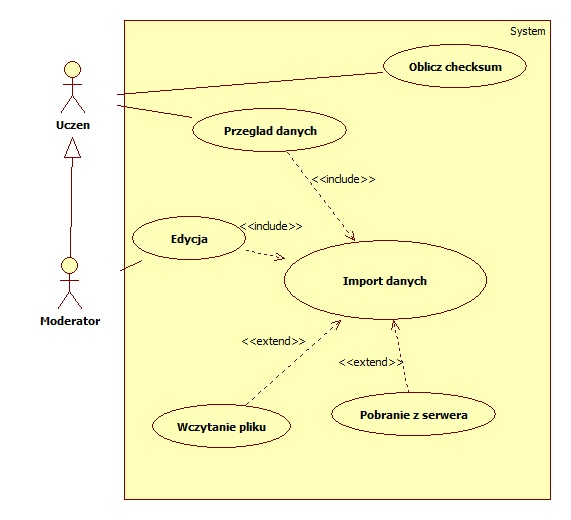
\includegraphics[width=120mm]{ge/caseuse.jpg}
  \caption{Case use.}
  \label{fig:caseuse}
\end{figure}

Niezwykle ważne jest aby pamiętać o strukturze aplikacji i ograniczeniach jakie niosą za sobą wykorzystane technologie. Każdy użytkownik uczeń według nomenklatury opisanej powyżej jest w posiadaniu pliku którego edycja powinna być zachowana jedynie dla moderatora. Niestety nie jest możliwe zapewnienie nieedytowalności pliku, z tego powodu nawet bez dostępu do uprawnień edycyjnych dostarczanych przez framework każdy może edytować plik w edytorze tektsowym, zmienić granice obszarów czy chociażby przedziały czasowe. Aby użytkownicy mieli pewność że plik z któego korzystają i mapa stworzona na jego podstawie jest wiarygodna i posiada poprawne dane proponowanym rozwiązaniem jest wykorzystanie jednego z algorytmu tworzących skrót z dowolnego ciągu danych, jednym z najczęściej wykorzystanym do takich celów jest MD5. Otrzymany wynik można zamieścić w widoczny miejscu obok pliku z danymi w miejscu gdzie jedynie moderator ma dostęp. Dzięki takiej operacji użytkownik będzie mógł porównać wygenerowany skrót pliku którego chce użyć z wartością na stronie, identyczne wartości potwierdzą autentyczność danych.

\subsection{Funkcje haszujące}
\label{sec:hashfunction}

W pewnych sytuacjach nie potrzebujemy lub nie chcemy przechowywać oryginalnego pliku lub ciągu znaków. Częstym wykorzystaniem jest utworzenie sktótu hasła w module logowania do różnych aplikacji. Czynność ta utrudnia poznanie rzeczywistych wartości w momencie dostępu do nich przez nieuprawnione osoby. Jedną z cech dobrej funkcji haszującej jest
spełnienie wymagań dla funkcji jednokierunkowej. Wymagane jest aby funkcja była łatwa do obliczenia ale trudna, lub wręcz niemożliwa do odwrócenia.
Do poznania wartości dla której został wygeneorany skrót można wykorzystać m.in. metodę słownikową, oznacza to wykonanie operacji haszującej dla dużego zbioru danych i odnalezienie szukanego sktótu w otrzymanych wynikach.

Innym częstym wykorzystaniem, zaproponowanym w poprzedniej sekcji, jest weryfikacja integralności pliku lub wiadomości. Umieszczenie w jedym miejscu pliku i jego skrótu umożliwia sprawdzenie czy plik który posiadamy jest identyczny z tym znajdującym się na stronie, w przypadku braku zgodności możliwe jest ściągnięci poprawnej wersji, w pozostałych sytuacjach posiadamy pewność autentyczności danych bez potrzeby każdorazowego ściągania pliku z serwera, oszcędzamy przez to czas poświęcony na ściągnięcie pliku, który może zajmować wiele megabajtów.

Istnieje wiele funkcji haszujących, wybór konkretnej z nich zależy od celu użycia najpopularniejszymy są MD5 i SHA-1.

\begin{itemize}
\item
MD5
Opracowany w 1991 roku przez Rona Rivesta, z dowolnego ciągu danych generuje 128-bitowy sktót,pozwala to na utworzenie 32 znakowego ciągu w systemie szesnastkwoym. Ważną cechą jest zmiana skróty w przypadku najmniejszej edycji wejściowych danych. Tabela \ref{tab:hashresult},stowrzona przy pomocy strony \underline{\texttt{http://www.sha1-online.com/}}, prezentuje przykład zmiany jednej litery, wygenerowany skrót dla tej wartości jest zupełnie inny.
Z uwagi na szybkość działania jest powszechnie używana, jednym z zastosowań jest ukrywanie haseł w bazie danych.

\item
SHA-1

Przedstawiciel funckji z rodziny SHA, opublikowany w 1995 roku. Wprzeciwieństiw do MD5 do zapisu skrótu korzysta z 160-bitów, oznacza do 40 znaków w systemie heksadecymalnym.

\item
SHA-2
Określenie czterech wariantów zastępujących SHA-1. Wersją zapewniającą najwyższą obecnie niezawodność i bezpieczeństwo jest SHA-512, do zapisu wykorzystuje 512 bitów co pozwala na otrzymanie 128 znakowego skrótu.

\end{itemize}

\begin{table}[H]
    \centering
    \begin{tabular}{|l|l|l|}
    \hline
    Algytm & Wejściowy ciąg & Wygenerowany skrót  \\ \hline
    MD5 & AGH Kraków &    c9c16a90d4938da799b5aa7d6f37edce  \\ \hline
    MD5 & AGH Krakow &    fc6a83206673002588490eb05b89313f  \\ \hline
    SHA-1 & AGH Kraków &  6205880f638b3e584578125b14231c30c3ab9fea  \\ \hline
    SHA-1 & AGH Krakow  & a536aa59ed829801cd0f099c4ae3ba34ca57ca9f \\ \hline
    SHA-512 & AGH Kraków &  49d9e2deb053a58dcb0a778758e5(...)61499145e36353  \\ \hline
    SHA-512 & AGH Krakow  & 6b65c56ca2e5567a5f18dd0d7465(...)f46166c29d7105 \\ \hline
    \end{tabular}
    \caption{Rezulaty funkcji haszujących}
    \label{tab:hashresult}
\end{table}

http://eprint.iacr.org/2008/469.pdf
